\documentclass[a4paper,oneside,14pt]{extreport}

\include{preamble}

\begin{document}
	\pagenumbering{Alph}

\begin{titlepage}
	\centering
	
	\begin{wrapfigure}[7]{l}{0.14\linewidth}
		\vspace{5mm}
		\hspace{-5.8mm}
		\includegraphics[width=0.93\linewidth]{images/bmstu-logo}
	\end{wrapfigure}
	{\singlespacing \footnotesize \bfseries Министерство науки и высшего образования Российской Федерации\\Федеральное государственное бюджетное образовательное учреждение\\высшего образования\\<<Московский государственный технический университет\\имени Н.~Э.~Баумана\\ (национальный исследовательский университет)>>\\(МГТУ им. Н.~Э.~Баумана)\\}
	
	\vspace{-2.2mm}
	\vhrulefill{0.9mm}\\
	\vspace{-7mm}
	\vhrulefill{0.2mm}\\
	\vspace{2mm}
	
	{\doublespacing \small \raggedright ФАКУЛЬТЕТ \hspace{2mm} \textbf{Информатика и системы управления}\\
		КАФЕДРА \hspace{2mm} \textbf{Программное обеспечение ЭВМ и информационные технологии (ИУ7)}\\
		НАПРАВЛЕНИЕ ПОДГОТОВКИ \hspace{2mm} \textbf{09.03.04 Программная инженерия}\\}
	
	\vspace{50mm}
	
	\textbf{ОТЧЕТ}\\
	\textbf{по лабораторной работе №1}\\
	{\doublespacing \small 
	\raggedright \textbf{Название:} \hspace{20mm}Расстояние Левенштейна\\
	
	\textbf{Дисциплина:} 
	\hspace{13mm} Анализ алгоритмов\\
	
	\vspace{50mm}
	
	{\singlespacing Студент: \hspace{20mm} \underline{ИУ7-55Б} \hfill 
	\underline{~~~~~~~~~~~~~~~~~}
	\hspace{5mm}
	\underline{М.~Н.~Серова}\\
	\hspace{40mm} {\tiny (Группа)}\hfill 
	{\tiny (Подпись, дата)~~}
	\hspace{7mm} {\tiny(И.~О.~Фамилия)~~~}\\}
	{\singlespacing Преподаватель:
		\hfill
		\underline{~~~~~~~~~~~~~~~~~}
		\hspace{5mm}
		\underline{Л.~Л.~Волкова}\\
	\hfill 
	{\tiny (Подпись, дата)~~}
	\hspace{7mm} {\tiny(И.~О.~Фамилия)~~~}\\} }
	
%	Оценка:        \hfill \hrulefill\\}
	
	\vfill
	
	Москва,	\the\year
	\thispagestyle{empty}
\end{titlepage}
\pagenumbering{arabic}
\newpage
\tableofcontents
\lstset{
	language = python,
	basicstyle=\small\sffamily,
	numbers=left,
	numberstyle=\tiny,
	stepnumber=1,
	numbersep=5pt,
	xleftmargin =.19in,
	showspaces=false,
	showstringspaces=false,
	showtabs=false,
	frame=single,
	tabsize=2,
	captionpos=t,
	breaklines=true,
	breakatwhitespace=false,
	escapeinside={\#*}{*)}
}

\newpage

\addcontentsline{toc}{chapter}{Введение}
\chapter*{Введение}

\textbf{Цель:} сравнить алгоритмы нахождения расстояния Левенштейна и Дамерау-Левенштейна.\\

\textbf{Задачи.}
\begin{enumerate}
	\item Изучить алгоритмы нахождения расстояния Левенштейна и Дамерау-Левенштейна.
	\item Реализовать алгоритмы:
	\begin{enumerate}
		\item рекурсивный алгоритм нахождения расстояния Левенштейна;
		\item матричный алгоритм нахождения расстояния Левенштейна;
		\item рекурсивный алгоритм нахождения расстояния Левенштейна с заполнением матрицы;
		\item расстояние Дамерау-Левенштейна.
	\end{enumerate}
	\item Применить методы динамического программирования для реализации алгоритмов.
	\item Провести сравнительный анализ алгоритмов по затрачиваемым ресурсам (времени и памяти).
\end{enumerate}
\newpage
\chapter{Аналитическая часть}
Расстояние Левенштейна~\cite{levenshtein} - минимальное количество редакторских операций, необходимых для преобразования одной строки в другую.
Редакторскими операциями являются:
\begin{itemize}
\item вставка (I - insert);
\item удаление (D - delete);
\item замена (R - replace);
\item совпадение (M - match).
\end{itemize}

В расстоянии Дамерау-Левенштейна дополнительно рассматривается операция перестановки соседних символов (X - exchange).
Для каждой редакторской операции задается своя цена (штраф). Следовательно, решение задачи нахождения редакционного расстояния сводится к нахождению минимальной суммарной цены всех проведенных для слов операций. Заметим, что для всех редакторских операций, кроме совпадения (M), штраф составляет 1.

Алгоритмы нахождения расстояния Левенштейна и Дамерау-Левенштейна применяются нескольких областях:
\begin{itemize}
\item в автокоррекции и автолингвистике (для автоматического исправления ошибок в слове, сравнении введенных слов со словарями в поисковых системах);
\item в биоинформатике (для сравнения генов, хромосом, белков).
\end{itemize}

\section{Рекурсивный алгоритм нахождения расстояния Левенштейна}
Пусть даны две строки $S_{1}$ и $S_{2}$ длиной M и N соответственно. Тогда расстояние Левенштейна можно вычислить по рекуррентной формуле \ref{eq1}, где D(i, j) - расстояние между строками $S_{1}[1..i]$ и $S_{2}[1..j]$, $S_{k}[i]$ - i-ый символ строки $S_{k}$.
\begin{equation} \label{eq1}
D(i,j) = \left \{ \begin{array}{ll}
0, \hfill i = 0,~j = 0\\
i, \hfill j = 0,~i > 0\\
j, \hfill i = 0,~j > 0\\
min \left\{ 
\begin{array}{ll}

\	\	D(i,j-1)+1,\\
\	\	D(i-1, j) +1, &\textrm{$j>0, i>0$}\\
\	\	D(i-1, j-1) + \left \{ \begin{array}{ll}
	0, & \textrm{если $S_{1}[i] = S_{2}[j]$}\\
	1, & \textrm{иначе}\\
	\end{array} \right. \\
	 %m(S_{1}[i], S_{2}[j])\\

\end{array} \right.
\end{array} \right.
\end{equation}
При этом очевидно, что верны следующие утверждения:
\begin{itemize}
	\item D($S_{1}, S_{2}$) $\geq$ ||$S_{1}$| - |$S_{2}$||;
	\item D($S_{1}, S_{2}$) $\leq$ max(|$S_{1}$|, |$S_{2}$|);
	\item D($S_{1}, S_{2}$) $= 0 \Leftrightarrow S_{1} = S_{2}$.
\end{itemize}
Рекурсивный алгоритм реализует формулу \ref{eq1}.

\section{Матричный алгоритм нахождения расстояния Левенштейна}

Прямая реализация формулы \ref{eq1} нахождения расстояния Левенштейна может быть малоэффективной при больших i, j, поскольку  промежуточные значения D(i, j) вычисляются повторно много раз. Для снижения затрат можно ввести матрицу для хранения соответствующих промежуточных значений - матрицу расстояний. В таком случае алгоритм представляет собой построчное заполнение матрицы $A_{m x n}$, элемент A[n][m] которой будет содержать итоговое расстояние Левенштейна.


\section{Рекурсивный алгоритм нахождения расстояния Левенштейна с заполнением матрицы}

Важный недостаток рекурсивной реализации алгоритма нахождения расстояния Левенштейна заключается в многократном вычислении  промежуточных значении D(i, j). Для оптимизации введем матрицу расстояний. Если рекурсивный алгоритм обрабатывает данные первый раз, полученное значение заносится в соответствующую ячейку матрицы, иначе используется уже вычисленное значение, и алгоритм переходит к следующему шагу.

\section{Расстояние Дамерау-Левенштейна}

Расстояние Дамерау-Левенштейна вычисляется по формуле, аналогичной \ref{eq1}, но с добавлением дополнительной операции. Таким образом, получим формулу \ref{eq2}.
\begin{equation} \label{eq2}
D(i,j) = \left \{ \begin{array}{ll}
0, \hfill $i = 0,~j = 0$\\
i, \hfill $j = 0,~i > 0$\\
j, \hfill $i = 0,~j > 0$\\
min \left\{ 
\begin{array}{ll}

\	\	D(i,j-1)+1,\\
\	\	D(i-1, j) +1, &\textrm{$j>0, i>0$}\\
\	\	D(i-1, j-1) + \left \{ \begin{array}{ll}
0, & \textrm{если $S_{1}[i] = S_{2}[j]$}\\
1, & \textrm{иначе}\\

\end{array} \right. \\
\	\	\left[ \begin{array}{ll}
D(i-2, j-2), &\textrm{если $i, j > 1$;}\\
&\textrm{$S_{1}[i] = S_{2}[j - 1]$;}\\
&\textrm{$S_{2}[j] = S_{1}[i - 1]$}\\
\infty, &\textrm{иначе}



\end{array} \right.
%m(S_{1}[i], S_{2}[j])\\

\end{array} \right.
\end{array} \right.
\end{equation}

Рекурсивная реализация данной формулы при больших значениях i, j будет работать долго по причинам, аналогичным рекурсивному алгоритму поиска расстояния Левенштейна, в связи с чем удобно ввести матрицу, аккумулирующую вычисленные значения.


\section{Вывод}
Формулы Левенштейна и Дамерау-Левенштейна для вычисления расстояния между строками задаются рекуррентно, что позволяет реализовать алгоритмы как рекурсивно, так и итерационно. Для оптимизации рекурсивных алгоритмов вводится вспомогательная матрица расстояний, хранящая промежуточные вычисления, она же применяется в итеративных алгоритмах.
\newpage
\chapter{Конструкторская часть}
Данный раздел содержит схемы алгоритмов, реализуемых в работе: Левенштейна и Дамерау-Левенштейна.
\section{Схемы алгоритмов нахождения расстояния Левенштейна}

На рисунке \ref{fig:rec_lev} представлена схема рекурсивного алгоритма нахождения расстояния Левенштейна.
\begin{figure}[H]
	\centering
	\includegraphics[width=1.05\linewidth, height=1.4\linewidth]{images/levenshtain_recursive}
	\caption{Схема рекурсивного алгоритма Левенштейна}
	\label{fig:rec_lev}
\end{figure}

На рисунке \ref{fig:iter_lev} представлена схема итеративного алгоритма нахождения редакционного расстояния между словами.
\begin{figure}[H]
	\centering
	\includegraphics[width=0.83\linewidth, height=1.3\linewidth]{images/iteratLevenshtain}
	\caption{Схема матричного алгоритма Левенштейна}
	\label{fig:iter_lev}
\end{figure}

Схема функции заполнения матрицы, вызываемой в итеративном алгоритме нахождения расстояния Левенштейна, представлена на рисунке \ref{fig:init_mat}.
\begin{figure}[H]
	\centering
	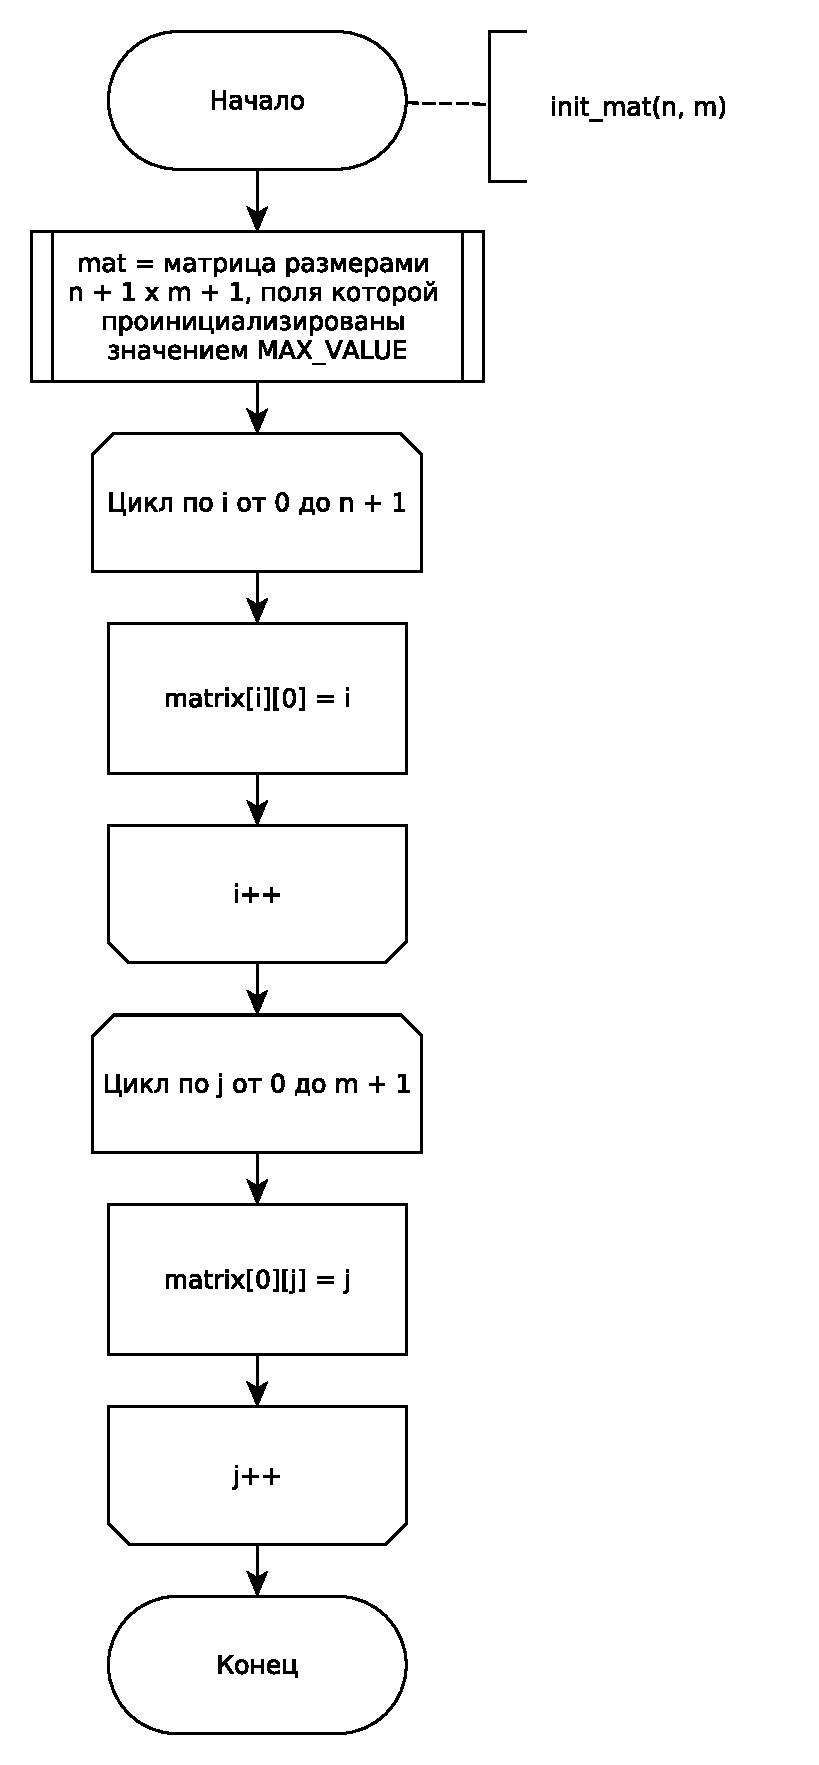
\includegraphics[width=0.59\linewidth]{images/init_mat}
	\caption{Схема функции, инициализирующей матрицу расстояний}
	\label{fig:init_mat}
\end{figure}


На рисунке \ref{fig:recur_lev_mat} представлена схема рекурсивного алгоритма нахождения расстояния Левенштейна с заполнением матрицы.
\begin{figure}[H]
	\centering
	\includegraphics[width=1.07\linewidth, height=1.2\linewidth]{images/recursLevenshtainMat}
	\caption{Схема рекурсивного алгоритма Левенштейна с кэшем}
	\label{fig:recur_lev_mat}
\end{figure}

\section{Схема алгоритма нахождения расстояния Дамерау-Левенштейна}

Схема алгоритма поиска расстояния Дамерау-Левенштейна представлена на рисунке \ref{fig:dam_lev}.
\begin{figure}[H]
	\centering
	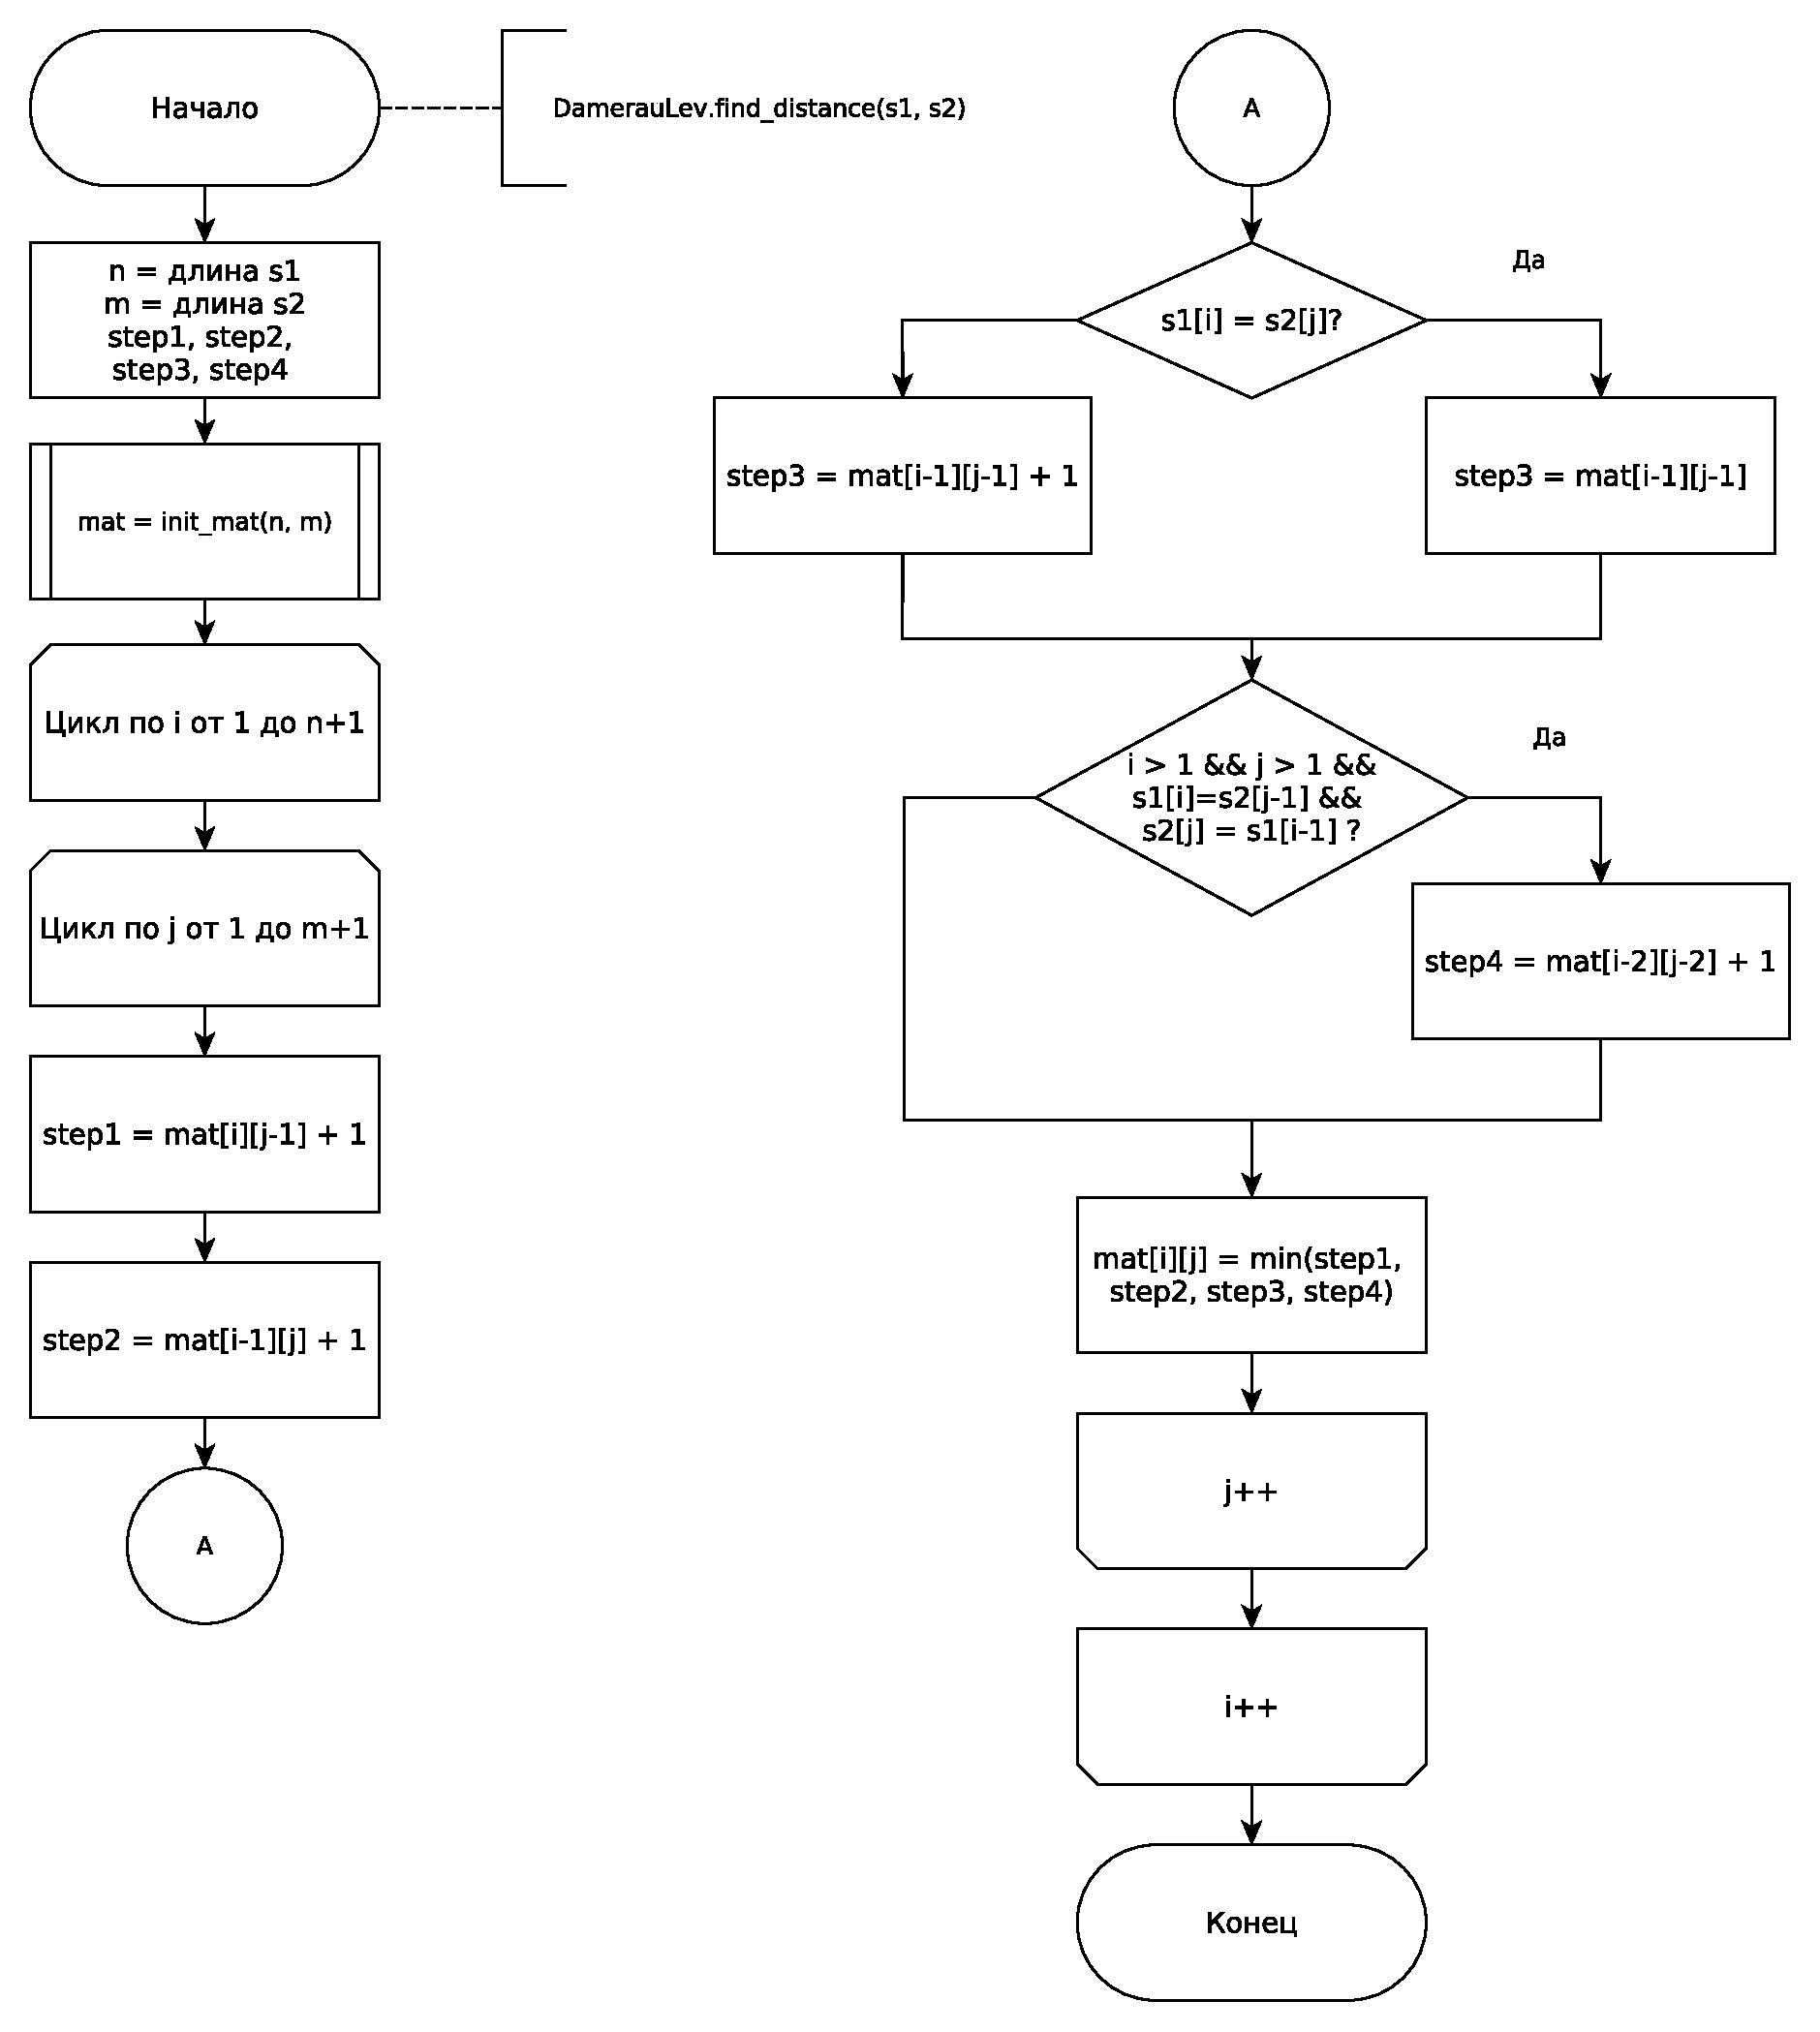
\includegraphics[width=1\linewidth]{images/damerayLevenshtain}
	\caption{Схема итерационного алгоритма Дамерау-Левенштейна}
	\label{fig:dam_lev}
\end{figure}

\section{Вывод}
В данном разделе на основе приведенных в аналитическом разделе теоретических данных были составлены схемы алгоритмов для реализации в технологической части.
\newpage

\chapter{Технологическая часть}
Данный раздел содержит обоснование выбора языка и среды разработки, реализацию алгоритмов.

\section{Требования к программному обеспечению}
Требования, выдвигаемые к разрабатываемому ПО:
\begin{itemize}
	\item входные данные - две строки $S_{1}$ и $S_{2}$ на английском или русском языках в любом регистре;
	\item выходные данные - искомое расстояние для всех алгоритмов.
\end{itemize}

\section{Средства реализации}
Для реализации программы был выбран язык программирования Python~\cite{python}. Такой выбор обусловлен следующими причинами:
\begin{itemize}
	\item данный язык программирования был освоен на практических занятиях;
	\item имеет большое количество расширений и библиотек, что облегчает работу с некоторыми типами данных и математическими формулами;
	\item обладает информативной документацией.
\end{itemize}

\section{Реализация алгоритмов}
В листингах \ref{lst:LevRec} - \ref{lst:Damerau} представлены реализации рассматриваемых алгоритмов.
\captionsetup{singlelinecheck=false}
\begin{lstlisting}[caption=Рекурсивный алгоритм вычисления расстояния Левенштейна (часть 1), label={lst:LevRec}]
class LevRecursive(StringDistanceFinder):
	def __init__(self):
		super().__init__()
	
	def find_distance(self, s1, s2):
		return self.__find_distance(s1, s2)
\end{lstlisting}
\begin{lstlisting}[caption=Рекурсивный алгоритм вычисления расстояния Левенштейна (часть 2), label={lst:LevRec}]
	def __find_distance(self, s1, s2):
		if len(s1) == 0:
			return len(s2)
		elif len(s2) == 0:
			return len(s1)
		D = self.__find_distance(s1[:-1], s2) + 1
		D = min(D, self.__find_distance(s1, s2[:-1]) + 1)
		m = 0 if s1[-1] == s2[-1] else 1
		
		D = min(D, self.__find_distance(s1[:-1], s2[:-1]) + m)
		
		return D

\end{lstlisting}

\begin{lstlisting}[caption=Матричный алгоритм вычисления расстояния Левенштейна, label={lst:LevMat}]
class LevIterative(StringDistanceFinder):
	def __init__(self):
		super().__init__()
	
	def find_distance(self, s1, s2):
		return self.__find_distance(s1, s2)
	
	def __find_distance(self, s1, s2):
		n = len(s1)
		m = len(s2)
		mat = self.init_matrix(n, m)
		for i in range(1, n + 1):
			for j in range(1, m + 1):
				step1 = mat[i][j - 1] + 1
				step2 = mat[i - 1][j] + 1
				elem = 0 if s1[i-1] == s2[j-1] else 1
				step3 = mat[i - 1][j - 1] + elem
				mat[i][j] = min(step1, step2, step3)
		return mat[-1][-1]
\end{lstlisting}
\newpage
\begin{lstlisting}[caption=Рекурсивный алгоритм вычисления расстония с заполнением матрицы, label={lst:LevRecMat}]
class LevRecursiveWithMat(StringDistanceFinder):
	def __init__(self):
		super().__init__()
	
	def find_distance(self, s1, s2):
		mat = self.init_matrix(len(s1), len(s2))
		return self.__find_distance(s1, s2, mat)
	
	def __find_distance(self, s1, s2, mat):
		i = len(s1)
		j = len(s2)
		if mat[i][j] != np.inf:
			return mat[i][j]
		if i == 0:
			return j
		if j == 0:
			return i
		D = self.__find_distance(s1[:-1], s2, mat) + 1
		D = min(D, self.__find_distance(s1, s2[:-1], mat) + 1)
		m = 0 if s1[-1] == s2[-1] else 1
		D = min(D, self.__find_distance(s1[:-1], s2[:-1], mat) + m)
		mat[i][j] = D
		return D
\end{lstlisting}
\newpage
\begin{lstlisting}[caption=Алгоритм Дамерау-Левенштейна, label={lst:Damerau}]
class DamerauLev(StringDistanceFinder):
	def __init__(self):
		super().__init__()
	
	def find_distance(self, s1, s2):
		return self.__find_distance(s1, s2)
	
	def __find_distance(self, s1, s2):
		n = len(s1)
		m = len(s2)
		mat = self.init_matrix(n, m)
		for i in range(1, n + 1):
			for j in range(1, m + 1):
				step1 = mat[i][j - 1] + 1
				step2 = mat[i - 1][j] + 1
				elem = 0 if s1[i - 1] == s2[j - 1] else 1
				step3 = mat[i - 1][j - 1] + elem
				step4 = np.inf
				if i > 1 and j > 1 and s1[i - 1] == s2[j - 2] and s2[j - 1] == s1[i - 2]:
					step4 = mat[i - 2][j - 2] + 1
				mat[i][j] = min(step1, step2, step3, step4)
		return mat[-1][-1]
\end{lstlisting}

\section{Тестирование}
В таблице \ref{tab:tests} представлены использованные для тестирования методом "черного ящика"\ данные, были рассмотрены все возможные тестовые случаи. Все тесты пройдены успешно. Здесь и далее "Рек.Лев."\ - рекурсивный алгоритм Левенштейна, "Ит.Лев."\ - матричный алгоритм Левенштейна, "Рек.Лев.(мат.)"\ - рекурсивный алгоритм Левенштейна с кэшем, "Д.-Лев."\ - итерационный алгоритм Дамерау-Левенштейна.
\newpage
\begin{table}[h]
	\begin{center}
		\captionsetup{justification=raggedleft, singlelinecheck=false}
		\caption[]{\label{tab:tests} Проведенные тесты}
		\begin{tabular}{|c|c|c|c|c|c|}
			\hline
			&                    & \multicolumn{4}{c|}{\bfseries Ожидаемый результат}    \\ \cline{3-4} \cline{4-5} \cline{5-6}\hline
			Строка 1& Строка 2 & Рек.Лев.&Ит.Лев.&Рек.Лев.(мат.)& Д.-Лев.\\ [0.5ex]
			\hline
			окно & компот & 4 & 4&4& 4\\
			\hline
			monarchy & democracy & 6 & 6& 6 & 5\\
			\hline
			  & text & 4 & 4 & 4 & 4\\
			\hline
			ура &   & 3 & 3& 3& 3\\
			\hline
			 &  & 0 & 0& 0 & 0\\
			\hline
			яичница & ячиинца & 3 & 3 & 3 & 2\\
			\hline
			adventure & time & 7 & 7 & 7 & 7\\
			\hline
		\end{tabular}
	\end{center}
\end{table}

\section{Выводы}
В данном разделе были реализованы и протестированы различные варианты алгоритма нахождения расстояния Левенштейна и итерационный алгоритм Дамерау-Левенштейна.
\newpage

\chapter{Экспериментальная часть}
В данном разделе сравниваются реализованные алгоритмы, дается сравнительная оценка затрат на память и время.

\section{Пример работы программы}
Пример работы программы представлен на рисунке \ref{fig:work_example}.
\captionsetup{singlelinecheck=true}
\begin{figure}[H]
	\centering
	\includegraphics[width=0.7\linewidth]{images/work_example}
	\caption{Демонстрация работы программы}
	\label{fig:work_example}
\end{figure}

\section{Технические характеристики}
Технические характеристики устройства, на котором выполнялось тестирование:
\begin{itemize}
	\item операционная система: Ubuntu 20.01 Linux x86\_64~\cite{ubuntu};
	\item оперативная память: 8 Гб;
	\item процессор: AMD Ryzen5 3500U~\cite{processor}.
\end{itemize}

\section{Время выполнения алгоритмов}

Время выполнения алгоритмов замерялось на автоматически генерируемых строках необходимой длины с использованием функции getrusage библиотеки resources~\cite{resource}. Усредненные результаты замеров процессорного времени приведены в таблице. Прочерк означает, что время ожидания значения результата превысило минуту, далее замеры не проводились. 
\begin{table}[h]
	\begin{center}
		\captionsetup{justification=raggedleft, singlelinecheck=false}
		\caption{\label{time} Время обработки строк разной длины в микросекундах}
		\begin{tabular}{|c c c c c|} 
			\hline
			Длина&Рек.Лев.&Ит.Лев.&Рек.Лев.(мат.)& Д.-Лев.\\ [0.5ex]
			\hline
			5  &  56193  &  1127  &  3171  &  1282 \\
			\hline
			7  &  1238515  &  1961  &  5723  &  2227 \\
			\hline
			10  & - &  2260  &  6884  &  2605 \\
			\hline
			20  & - &  8449  &  27139  &  9911 \\
			\hline
			50  & - &  51052  &  167683  &  61132 \\
			\hline
			100  & - &  203366  &  668480  &  244068 \\
			\hline
		\end{tabular}
	\end{center}
\end{table}

\begin{figure}[H]
%	\centering
	\includegraphics[width=1\linewidth]{images/lev_graph}
	\caption{Сравнение времени работы алгоритмов Левенштейна}
	\label{fig:lev_graph}
\end{figure}


\begin{figure}[H]
	\centering
	\includegraphics[width=1\linewidth]{images/dam_lev_graph}
	\caption{Сравнение времени работы алгоритмов Левенштейна}
	\label{fig:dam_lev_graph}
\end{figure} 

\section{Использование памяти}

С точки зрения использования памяти алгоритмы Левенштейна и Дамерау-Левенштейна отличаются незначительно. Поэтому для оценки использования памяти достаточно рассмотреть разницу рекурсивной и матричной реализаций алгоритмов.

Нагрузка функции на память состоит из следующих частей:
\begin{itemize}
\item аргументы - две строки - $2 * sizeof(string)$;
\item локальные переменные -целочисленная переменная - sizeof(int);
\item переменная с ответом - целочисленная переменная - sizeof(int);
\item адрес возврата - addr.

\end{itemize}

Важно учесть, что максимальная глубина стека будет соответствовать сумме длин входных строк: sizeof($S_{1}$) + sizeof($S_{2}$). 

Таким образом, общее количество памяти, затрачиваемое рекурсивным алгоритмом, можно вычислить по формуле \ref{eq:rec_memory}.
\begin{equation} \label{eq:rec_memory}
	\begin{array}{ll}
	M_{recursive} = (sizeof(S_{1}) + sizeof(S_{2})) \cdot (2 \cdot sizeof(string) +\\
	+ 2 \cdot sizeof(int) + addr)
	\end{array}
\end{equation} 

Для вычисления объема используемой памяти при матричной реализации алгоритма используется формула \ref{eq:mat_memory}.
\begin{equation} \label{eq:mat_memory}
	\begin{array}{ll}
	M_{matrix} = (len(S_{1}) + 1) \cdot (len(S_{2}) + 1) \cdot \\
	\cdot sizeof(int) + 2 \cdot sizeof(string) + 9 \cdot sizeof(int) + addr
	\end{array}
\end{equation}

Для рекурсивного алгоритма с заполнением матрицы необходимо учесть дополнительные затраты на хранение матрицы и передачу ее в качестве аргумента. Таким образом получим формулу \ref{eq:rec_mat_memory} для вычисления затрат по памяти на выполнение рекурсивного алгоритма с матрицей.
\begin{equation} \label{eq:rec_mat_memory}
	\begin{array}{ll}
	m_{mat} = (len(S_{1}) + 1) \cdot (len(S_{2}) + 1) \cdot sizeof(int)\\
	M_{recurs-with-matrix} = (sizeof(S_{1}) + sizeof(S_{2})) \cdot \\
	\cdot (2 \cdot sizeof(string) + 4 \cdot sizeof(int) + addr + m_{mat}) + m_{mat}
	\end{array}
\end{equation}

\section{Выводы}

Рекурсивная реализация алгоритма нахождения расстояния Левенштейна работает дольше других более чем в 40 раз за счет большого количества повторяющихся вычислений, причем время работы возрастает в 2 раза при увеличении длины входных строк на 2. Итерационные реализации алгоритмов Левенштейна и Дамерау-Левенштейна сопоставимы по времени выполнения. Рекурсивный алгоритм Левенштейна с заполнением матрицы работает быстрее обычного рекурсивного, но в три раза медленнее обеих матричных реализаций.

Однако итеративные алгоритмы менее эффективны по памяти за счет необходимости хранения матрицы, размерность которой превышает на 1 длину строк. Таким образом, если для рекурсии количество памяти возрастает пропорционально сумме длин строк, то для матричного алгоритма - пропорционально их произведению.
\newpage

\addcontentsline{toc}{chapter}{Заключение}
\chapter*{Заключение}
В процессе выполнения лабораторной работы были изучены алгоритмы поиска расстояния Левенштейна и Дамерау-Левенштейна. Получен практический навык реализации этих алгоритмов в итерационной версии, алгоритма Левенштейна в рекурсивной и рекурсивной с заполнением матрицы версиях.

Были исследованы процессорное время выполнения и затраты на память выше обозначенных алгоритмов. В результате было выявлено, что дольше всего выполняется рекурсивный алгоритм Левенштейна (более чем в 40 раз дольше других), быстрее всего - итерационный алгоритм Левенштейна, при этом время выполнения итерационного алгоритма Дамерау-Левенштейна сопоставимо с аналогичной версией алгоритма Левенштейна. 

На основе кода были получены формулы для вычисления использованной памяти для каждой версии алгоритмов. Согласно полученным выражениям, матричные алгоритмы значительно проигрывают по памяти рекурсивным за счет необходимости хранения вспомогательной матрицы.


\newpage
\addcontentsline{toc}{chapter}{Список литературы}

\bibliographystyle{utf8gost705u}
\bibliography{bib_lab_1}
\nocite{*}



\end{document}